%!TEX root =  main.tex
\chapter{Micro clouds and edge computing as a service}\label{chapter:Micro_clouds}
%
This section explains the model of EC as a service compared to the traditional CC model. We present the formation of such a system with a formal model and proof of concept implementation based on the proposed model.

In Section~\ref{sec:configurable_model_structure} present configurable model used to describe our system. in Section~\ref{sec:separation_of_concerns} we present separation of concerns for our model. In Section~\ref{sec:as_a_service_model} we discuss how this system could be offered as a service model and could be used for EC as a service. In Section~\ref{sec:application_model} we present possible application model and how users can utilize newly created architecture fully, using existing application models. Section~\ref{sec:immutable_infrastructure} present desired option for infrastructure deployment. In Section~\ref{sec:formal_model} we present why formal models are important in computer science and DS in particular, as well as model of our system with all protocols and nodes properties. Section~\ref{sec:repercussion} give repercussion of proposed model, and how it can be used as stand alone model where other features could be implemented on top of that or used as service for other, existing, systems. Finally, section~\ref{sec:limitations} present limitation of our model.
%
%
\section{Configurable Model Structure}\label{sec:configurable_model_structure}
%
Satyanarayanan et al.~\cite{SatyanarayananK19} propse architecture eparated into 3 tiers. Combained with MDCs and a zone-based server organization we get a good starting point for building EC as a service and micro cloud system, because we can extend the computing power and storage capacity serving local population. But, we need a more available and resilient system with less latency. To do that we need to extend these concepts and adopt them for different usage scenario.

If we take a look at the CC design, every part contributes to a more resilient and scalable system. Regions (or DCs) are isolated and independent from each other, and also contain resources application needs. They are usually composed of few availability zones~\cite{SouzaMFAK19}. If the one zone fails, there are still more of them to serve user requests. With some adaptations, EC could use a similar proven strategy. That strategy could be than used in applications beyound just EC.

Table~\ref{tab:table5} shows similar concepts between CC and edge centric computing (ECC) concepts, with accent on difference what is the physical part, and what are logical concepts.

\begin{table}[h!]
	\begin{center}
		\begin{tabular}{l|l}
			\textbf{Edge centric computing} & \textbf{Cloud computing}\\
			\hline
			Topology (logical) & Cloud provider (logical)\\
			Region (logical) & Region (physical)\\
			Cluster (physical) & Zone (physical)\\
		\end{tabular}
	\end{center}
	\vspace{-0.5cm}
	\caption{Similar concepts between cloud computing and ECC.}
	\label{tab:table5}
\end{table}

We can combine multiple node clusters into a bigger logical concept of $region$, increasing availability and reliability of both system and applications. We are talking about geo-distributed systems, so we have a bit of a different scenario than in the standard CC model. The cloud region is a physical thing~\cite{SouzaMFAK19}, while in the ECC a region could be represented in a different way. We now give a forma definition of a $region$ in ECC as:

\begin{definition}
	In geo-distributed ECC and micro clouds, a regoin is used to describe a set of clusters over an arbitrary geographic region. 
\end{definition}

Regions can accept or release clusters and clusters can accept or release nodes. Based on this property, we can define minimum size of an ECC region as:

\begin{definition}
	ECC regions are composed of at least one cluster, but can be composed of much more, so as to achieve a more resilient, scalable, and available system. 
\end{definition}

To ensure less latency in the system, vast distance between clusters should be avoided in normal circumstances. In a CC, region extension requires physically connecting modules to the rest of the infrastructure \cite{Hamilton07}.\\ 

Multiple regions form a second logical layer - $topology$. Formaly, we can define a $topology$ in ECC as:

\begin{definition}
In geo-distributed ECC and micro clouds, topology is a logical concept composed of a minimum one region, and could span over more regions. 
\end{definition}

When designing a topology, especially if regions need to share information, vast distance between regions should be avoided, if possible. With these simple abstractions, we can cover any geographic region with the ability to shrink or expand clusters, regions, and topology. Separation on $clusters$, $regions$, and $topologies$ is a matter of agreement and usages similar to modeling in Big Data systems~\cite{SonbolOAA20, WangCAL14}. 

For example, clusters could be as wide as the whole city or small as all devices in a single household and everything in between. The city could be one region with parts of the city being organized into clusters. We can form a city topology by splitting the city into multiple regions containing multiple clusters, or we can form a country topology by splitting the country into regions, with cities being regions. We can follow a more natural administrative division of some region, and organize resources by population usages.

Nodes inside the cluster should run some membership protocol. Gossip style protocols, like SWIM~\cite{DasGM02}, could be used in conjunction with replication mechanisms~\cite{LiBCL20, CauCBFCEB16,CRDTS_Nuno} making the whole system more resilient. In~\cite{inproceedingsSimic2} Simi\' c et al. take a look from theoretical point of view on conflict free replicated data types (CRDTs) usage, to achieve SEC in EC and conclude that CRDTs could be natural fit to EC as long as we are aware of potential pitfals of CDRTs.

Single $topology$ reflects one CC provider, so multiple $topologies$ are forming $micro-clouds$ that are able to help CC with huge latency issues, pre-processing in huge volumes of data and relax and decentralize strict centralized CC model.

These micro-clouds have much less resources, copared to standard clouds but they are much closter to the user meaning they have much fater response. In case of storage, if data is not present in the time of user request, they can pull data from the cloud and cache it for latter.

This 3 thier acrchitecture with numerous clients in the bottom, micro clouds in the middle, and cloud on the top kinda resembles cache level architecture in CPU~\cite{FarshinRMK19}. 

On lower levels we have fastest response time, since data is on the device. But at the same time, we have very limited storage capacity and processing power. As we go on the upper tiers, we have more and more storage capacity and processing power, but contrary the response time is higher and higher.  Esspecially when we take distance into consideration, and huge volumes of data that need to be moved to the cloud.

Figure~\ref{fig:fig9}. shows the 3 tier architecture, with the response time and resource avelability.

\begin{figure}[H]
	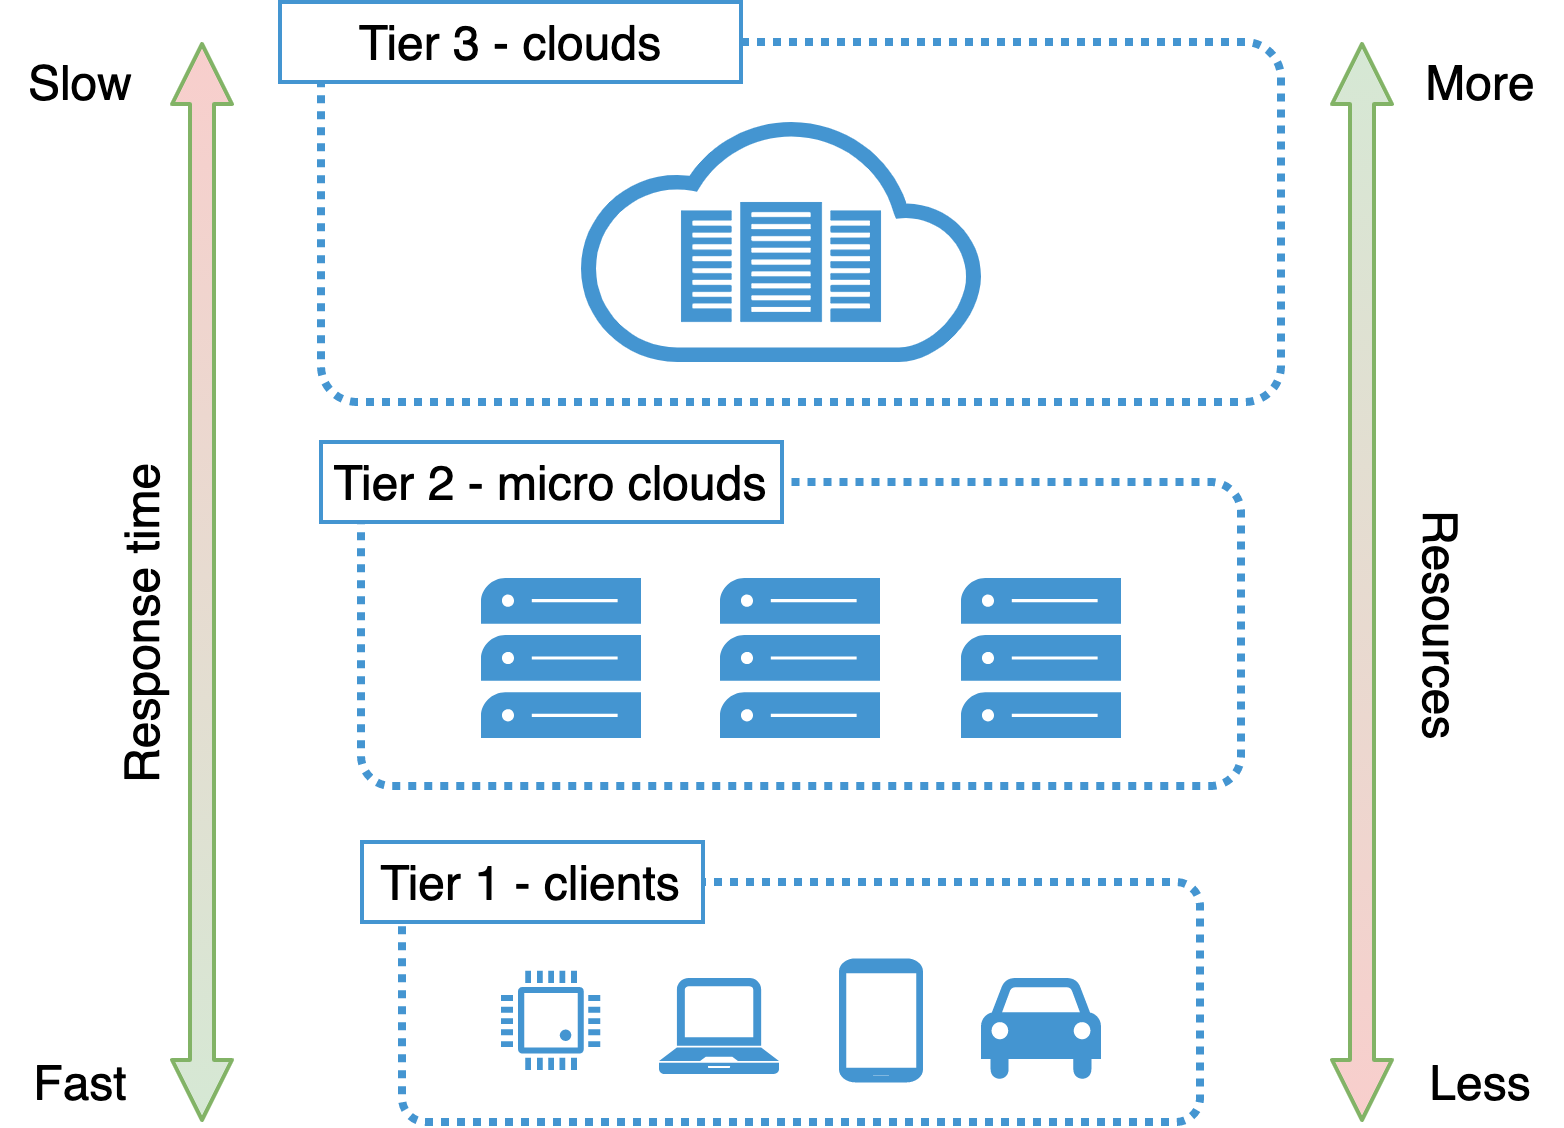
\includegraphics[width=\linewidth]{images/Figure9}
	\vspace{-0.7cm}
	\caption{3 tier architecture, with the response time and resource avelability}
	\label{fig:fig9}
\end{figure}

In everything as a service model~\cite{DuanFZSNH15}, EC as a service fits in between CaaS and PaaS, depending on users needs. 
%
%
\section{Separation of concers}\label{sec:separation_of_concerns}
%
To describe physical services, Jin et al.~\cite{JinCJL14} proposes three core concepts and specifies their relationships. These concepts are: $(1)$ Devices, $(2)$ Resources, and $(3)$ Services. 

SoC is a vital part of any system, especially if creating a platform to offer as a service. We based our SoC model for ECC as a service on these concepts, with adaptations for our use case, separated in three layers depicted in Figure~\ref{fig:fig10}. 

The first or bottom layer consists of various devices, and these devices represents \textit{data creators} and \textit{services consumers}. 

The second layer represents resources. Resources have a spatial features, and they indicate the range of their hosting devices~\cite{JinCJL14}. Developers at any time must know topology, the resource utilization and spread, as well as application's state and health.~\label{soc:resources}

Resources represent EC nodes, and to be part of the system, a node must satisfy four simple rules:

\begin{enumerate}[start=1,label={(\bfseries \arabic*)}]
\item run an operating system with a file system 
\item be able to run some application isolation engine, for example a container or unikernels 
\item have available resources for utilization 
\item have stable internet connection
\end{enumerate}

Services expose resources through an interface and make them available on the Internet~\cite{JinCJL14}. These services respond to clients immediately if possible, or cache information~\cite{SatyanarayananBCD09,YaoXWYZP20} for future requests. Services in the cloud should be able to accept pre-processed data, and they are responsible for computation and storage that is beyond the capabilities of ECC nodes. Services in the cloud should be able to take direct requests from client just in case that something catastrific happend to the micro-cloud that is close to the user.

Figure~\ref{fig:fig10}. shows the proposed SoC for every layer of the ECC as a service model.

\begin{figure}[H]
	\includegraphics[width=\linewidth]{images/FIG1}
	\vspace{-0.7cm}
	\caption{ECC as a service architecture with separation of concerns.}
	\label{fig:fig10}
\end{figure}
%
%
\section{As a service model}\label{sec:as_a_service_model}
%
Users should be able to develop their applications using two different models:
 
\begin{enumerate}[start=1,label={(\bfseries \arabic*)}]
	\item \textbf{microPaaS or mPaaS}, where the platform is doing all the management and offers a simple interface for developers to deploy their applications. This model is similar to PaaS, and the only difference is that this is running in micro-cloud and synchronize with CC.
	\item \textbf{microCaaS or mCaaS}, if users require more control over resources requirements, deployment and orchestration decisions. This model is similar to CaaS, and the only difference is that this is running in micro-cloud and synchronize with CC.
\end{enumerate}

Both variants should not stand alone, at least not for now. Fot that same reason we do not have microSaaS or mSaaS option, since that woul requre that whole application is running \textbf{only} in micro-clouds. But both options could be included, and part of any cloud model presented in~\ref{sec:cloud_computing}, or offered separatly.
%
%
\section{Applications Model}\label{sec:application_model}
%
Traditional DCs and CC propose specially designed cloud-native applications~\cite{GannonBS17}, that are easier to scale, more available, and less error-prone when compared to traditional web applications~\cite{GannonBS17}. Edge-native applications~\cite{SatyanarayananK19} should use the full potential of EC infrastructure, and keep good features of their cloud counterparts. 

Applications may be split in front and back processing services. Front processing service is an edge-native application running inside micro cloud to minimize latency, while the back service runs in traditional cloid as a cloud-native application to leverage greater resources. 

These edge-native applications will handle user requests coming to nearby MDCs, and communicate to cloud-native applications when needed. Separation like that gives developers better flexibility and large design space. 

With this model we venture even deeper into understanding and applying concept of \textbf{data locality} presented on page~\pageref{ds:data_locality}. Since we have split into front and bakc processing, we are committed to do processing data closer to their soruce, instead of moving data to the cloud. But restriction is that, at the moment, these EC nodes are not equiped with huge processing and storage capacity. But nonetheless, we are moved processing even closer to the data, instead moving huge volumes of data to computing. This is most important part of the data locality.
%
%
\subsection{Execution models}\label{sec:execution_models}
%
Frontend services model should be packed in some standard way~\ref{sec:virtualization_techniques} and deployed in the wild, as an event-driven applications, with the subscription policy to message streams, or infinite sequences~\cite{Rutten03} using topics~\cite{inproceedingsBeck}. The processing strategy is in the developer's hands, depending on the nature of the use-case. 

If an services are subscribed to some stream using topic for example, it is naturally that events apear in their stream. There are basically two strategies for building a large-scale time-ordered event system:

\begin{enumerate}[start=1,label={(\bfseries \arabic*)}]
	\item \textbf{Fan out on write}, with this strategy every service has some form of inbox, and when event apear for some topic, that data is copied to every service that is subscribed. With this options, deads are fast, but writes are not because the more followers to the topic the longer it takes to persist all updates. 
	\item \textbf{Fan in on read}, with this strategy every topic have a sort of outbox where it can store data. When services read their streams, the system will read the recent data from the outboxese. Writes are fast, and used storage is minimal, but reads are difficult because to do this properly on request-response deadline is not a trivial task to do.
\end{enumerate}

\noindent 
to implemente those ideas withoout comlicated synchronization CRDTs could be used~\ref{crdts}, as companies like Soundcloud laready are using them for the same or similar tasks.

Some examples of applications may include:

\begin{enumerate}[start=1,label={(\bfseries \arabic*)}]
	\item \textbf{events} that notify users if some value is above or below some defined threshold; 
	\item \textbf{stream} or processing data as it comes to the system;
	\item \textbf{batch} does processing in predefined times over some bigger collection of data ;
	\item \textbf{daemons} or processing that are doing some tasks or executions in the backgound without explicit user intervention, usually they their execution could be time defined but it is not mandatory;
	\item \textbf{services} or applications that would operate over standard request-response model or some variantion of that protocol. For example NATS messageing system have request-replay form implemented over topics;
	\item \textbf{other}, something that falls outside these models, or it is composition of multiple operations at once. This type should get events from some topic as they arrive, and user can define his own strategy what it needs to be done and how it needs to be pcessed. Usec can contact other existing services, and user is responsabile for optimization;
\end{enumerate}

These types of applications could be implemented in may ways like those disccused in~\ref{sec:microservices}, or some adapted variant of those models, and should have clear communicatoin interface offered to users or applications and other services.
%
\subsection{Packaging options}\label{sec:packaging}
%
Because their nature, micro clouds could be most likley composed of ARM devices. These devices in many cases are not able to run full VMs because their hardware restrictions. In recent years there are advances in VMs technology and their ability to run VMs on ARM devices. In~\cite{Ding12armvisor} Ding et al. show such possibility to run VMs on ARM devices.

But even if VMs are fully compatable with ARM devices, we still inherite VMs large footprint, already descused in~\ref{sec:virtualization_techniques} if we try to use tham $as is$.

On contrary, containers and unikernels give us $more for less$ same functionality but using less resources, meaning we can run more services in containers and even more in unikernels. But untill unikernels are fulkly ready to be used they will fall in nice to have category, and we should stick to containers. But even with containers we need to be aware of their limitations and pitfalls, and know that there is no $silver bullit$ and there is no one solution for all scenarios.

At the moment, containers are more matured solution than unikernels, and require less resources than VMs. On top of that, there are numerous of tools already existing using containers that could be utilized. Knowing all this, at first stages of micro-clouds, containres should be option to go. 

In~\cite{inproceedingsSimic3} Simi\' c et al. show benefits of using containres in large sclae edge computing systems from theoretical point of vew, by looking into architecture difference. Authors focus on differences between VMS and containers in cases where services needs to be runned on ARM devices with limited resources.

In future and when unikernels are more matured and tested, they could be used for paritical use-cases and applications, esspecially like events or serverless implementations. Containres will probably not be fully replaced, but they can co-exist with unikernels in some cases where we need more controll over running single function.

Like any other system, users can create their own variants of the systems and different flavours optimized for certen solutions. In that cases, they may favorized one solution over the other one. But in general case containers and unikernels should be prefered way to package, run and distributed user applicatoins in micro-clouds environment.
%
%

\section{Immutable infrastructure}\label{sec:immutable_infrastructure}
%
As described in~\ref{sec:deployment}, we have few options when it comes to setup and deply infrastructure and/or applications. This thesis propose DS model that is build with three tier architecture that should operate in geo-distributed environment we blieve that \textbf{immutable deployment} model would be good fit. It will simplify deployment process, since we want to rely on atomic operations and do not want to left misconfigured system at any level. If something like that happend, we will end up in problem, that would be hard to properly address and resolve.

Geo-distributed micro-clouds model that is described in this chaper, should operate in two levels of deployment that are build one on top of the another:

\begin{enumerate}[start=1,label={(\bfseries \arabic*)}]
	\item \textbf{Infrastructure deployement}, update and change should be atomic and immutable. Users should do changes declaratively --- mutations of the system, by telling the system what new state should be, and let the system to figure out the best way how to do user specified changes. In this category, we can account any change that is doing on the cluster, region or topology that user/s operate on. For example create of new cluster, region, topology or doing configurations of the setup system. The only change that could possible be done by imperative strategy is updates on the nodes itself. But even for this strategy, it would be beneficial if we could usedeclarative way \textbf{if possible}. It is important to notice that \textbf{mutation} does not mean in place change, but just name of operation. This deployment strategy is reserved for operations people, but if compay or team is small any developer could do this. Developers should not be dealing with this part of the deployment.
	\item \textbf{Services deployment}, make sense only if previous action is takane. We must have infrastructure setup already, in order do put any sort of services (applications) into the system. As previous model, this should be done declaratively as well, and all changes dould be done immutably without any in place change. User should specify his new state or \say{view of the word} declaratively and let system do all the changes he wants. All user services should be packed as described in~\ref{sec:packaging} because this simplifies way services are put to the nodes. When done properly, this allow operations people to do faster changes with almost zero downtime deployments with all strategies already discused in~\ref{sec:deployment}. this part of the deployemnt should be done by developers, since they done implementation and testing. They know hos much resources they need for their service, what type of service they had developed. This deployment could be done in colaboration between operations and deveopers, if compay is big or time is properly separated.
\end{enumerate}

It is important to notice, that both deployments should be closley followed, for posible errors and problems so that users can act accordingly. This deployment messages, logs and traces should be stored in centralized log system, for convenient lookup, alerting and reporting.

Separation like this, simplify deployment and usage for both application development spectrums: 

\begin{enumerate}[start=1,label={(\bfseries \roman*)}]
	\item operation people like \textbf{devops} who should be dealing with infrastructure deployment, tooling setup, applications deployment, monitoring and in general health of applications and infrastructure.
	\item \textbf{developers} who should be dealing with development of the services, their interactions, and cloud to micro cloud and vice-verca synchrnonizations.
\end{enumerate}

Only with tight colaboration with those two development roles, such complex system like one presetned in this chapter can be alive, well and servig user requests withoyt collaps.
%
%
\section{Formal model}\label{sec:formal_model}
%
Ensuring reliability and correctness of any system is very difficult, and should be mathematically based. Formal methods are techniques that allow us specification and verification of complex (software and hardware) systems based on mathematics and formal logic. There are several options how to formaly describe DS: TLA+, $pi$ calculus, combinational topology, asynchronous session types (MST), etc. 

Unfortunately, becasue of their nature DS cannot always be formally described by any of the existing models. But if the nature of the DS that is developing is such that can be formaly described, it is recomended and beneficial. Formaly described and corect model, can save hours, days and event months of hard debugging, testing to reveal all bugs and problems in the system.

Infrastructure deployment will not happen until the process is trivial \cite{SatyanarayananBCD09}, hence the key is to simplify ECC management. The main problem is that going to every node is tedious and time consuming, especially in a geo-distributed environment. In such complex environemnt, formal models are of great help if we can model and prove that protocols that system reyls on are correct. The system we propose tackles this issue using remote configuration and it relies on four formaly modeled protocols: 

\begin{enumerate}[start=1,label={(\bfseries \arabic*)}]
	\item \textbf{health-check} protocol informs the system about state of every node (cf. Section~\ref{sec:health_check_protocol})
	\item \textbf{cluster formation} protocol forms new clusters dinamicaly (cf. Section~\ref{sec:cluster_formation_protocol})
	\item \textbf{idempotency check} protocol for preventing creating existing infrastructure (cf. Section~\ref{sec:idempotency_protocol})
	\item \textbf{list detail} protocol shows the current state of the system to the user (cf. Section~\ref{sec:list_detail_protocol})
\end{enumerate}

These three protocols are base of the geo-distribued Infrastructure deployment.

In Section~\ref{sec:multiparty} we give short introduction what MST are and what properties they guarantee. Section~\ref{sec:health_check_protocol} describe formal model of healh-check protocol. Section~\ref{sec:cluster_formation_protocol} describe cluster formation protocol. Section~\ref{sec:list_detail_protocol} describe protocol that return data based on some query.
%
%
\subsection{Multiparty asynchronous session types}\label{sec:multiparty}
%
We can model communication protocols %from node to the system 
using~\cite{HuY17}, an extension of \emph{multiparty asynchronous session types} (MPST)~\cite{HondaYC08} %, HondaYC16} 
--- a class of behavioral types tailored for describing distributed protocols relying on asynchronous
communications. 

The type specifications are not only useful as formal descriptions of the protocols, but we can also rely on a modeling-based approach developed in~\cite{HuY17} to validate our protocols satisfies multiparty session types safety (there is no reachable error state) and progress (an action is eventually executed, assuming
fairness). %\comment{Mozda ovo naglasiti jos od samog uvodjenja tipova sesija??}

The first step in modeling the communications of a system using MPST theory 
is to provide a \emph{global type}, that is a high-level description of the overall protocol from the neutral 
point of view. 
Following~\cite{HuY17}, the syntax of global types is constructed by:

\begin{equation}
	\G \; ::= \;
	\{\pp\dagger\pq_i{:}\ell_i(\T_i).\G_i\}_{i\in I}  \quad | \quad 
	\mu \ty.\G \quad | \quad 
	\ty \quad | \quad
	\tend
\end{equation}
\myequations{Global type construction}

where $\dagger\in\{\to, \twoheadrightarrow\}$ and $I\not=\emptyset$. 
In the above, $\{\pp\dagger\pq_i{:}\ell_i(\T_i).\G_i\}_{i\in I}$
denotes that \emph{participant} $\pp$ can send (resp. connects) to one of the participants $\pq_i$, 
for $\dagger=\to$ (resp. $\dagger=\twoheadrightarrow$), 
a \emph{message} $\ell_i$ with the \emph{payload} of \emph{sort} $\T_i$, 
and then the protocol continues as prescribed with $\G_i$.  
$\mu \ty.\G_1$ is a recursive type, and $\ty$ is a recursive variable, 
while $\tend$ denotes a terminated protocol. We assume all participants are (implicitly) disconnected at the end of each session (cf.~\cite{HuY17}). 

The advance of using approach of~\cite{HuY17}, when compared to standard MPST (e.g.,~\cite{HondaYC08}),
is in a relaxed form of choice (a participant can choose between sending to different participants), 
and, $\twoheadrightarrow$, that explicitly connects two participants, hence (possibly) dynamically 
introducing participants in the session.
Both of these features will be significant for modeling our protocols (we will return to this point).

The second step in modeling protocols by MPST is providing a syntactic projection of the protocol onto each participant as a local type, that is then used to
type check the endpoint implementations.  
We use the definition of projection operator given in~\cite[Figure \ref{fig:fig2}]{HuY17}. 
In essence, the projection of global type $\G$ onto participant $\pp$ can result in 
$\ST_\pp=\pq{!}\ell(\T)\ldots$ (resp. $\ST_\pp=\pq{!!}\ell(\T)\ldots$) 
when $\G=\pp\to\pq{:}\ell(\T)\ldots$ (resp. $\G=\pp\twoheadrightarrow\pq{:}\ell(\T)\ldots$), 
and, dually, $\ST_\pp=\pq{?}\ell(\T)\ldots$ (resp. $\ST_\pp=\pq{??}\ell(\T)\ldots$) when $\G=\pq\to\pp{:}\ell(\T)\ldots$ 
(resp. $\G=\pq\twoheadrightarrow\pp{:}\ell(\T)\ldots$), 
while the projection operator ``skips'' the prefix of a global type if participant $\pp$ is not mentioned neither as sender nor as receiver. Furthermore, a local type must be represented by the following syntax:

\begin{equation}
	\ST \; ::= \; 
	{+}\{\pq_i\alpha\ell_i(\T_i).\ST_i\}_{i\in I}  \quad | \quad 
	\mu \ty.\ST \quad | \quad 
	\ty \quad | \quad
	\tend
\end{equation}
\myequations{Local type representation syntax.}

where $\alpha\in\{{!}, {!!}\}$ or  $\alpha\in\{{?}, {??}\}$ (in which case $\pq_i=\pq_j$ must hold for all $i,j \in I$, to ensure consistent external choice subjects, cf.~\cite[Page 6.]{HuY17}), and $I\not=\emptyset$.
Interested reader can find details in~\cite{HuY17}.

For simplicity, we consider all participants are communicating within a single private session, and that all sent messages, but not yet received, are buffered in a single queue that preserves their order. 

Actually, the order is preserved only for pairs of messages having the same sender and receiver, while other pairs of massages can be swapped, since these are asynchronously independent.
%
%
\subsection{Health-check protocol}\label{sec:health_check_protocol}
%
In a clustered environment, every node has a channel where it sends metrics, as a health-check mechanism. We can use this channel or create a new one to spread actions to the nodes, for example, a cluster formation message. 

Figure \ref{fig:fig6}. shows a low-level health-check protocol between a single node and the rest of the system, involving the following participants: Node, Nodes, State, and Log.

\begin{figure}[H]
	\begin{center}
		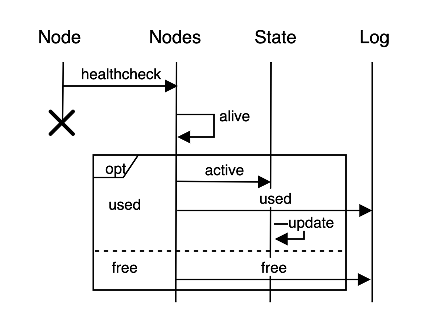
\includegraphics[scale=0.75]{images/FIG2}
	\end{center}
	\vspace{-0.7cm}
	\caption{Low level health-check protocol diagram.}
	\label{fig:fig6}
\end{figure} 

The participants which are included in Figure \ref{fig:fig6} follow the next protocol:\label{informal_description_health-check} that is described informally below:

\begin{enumerate}[start=1,label={(\bfseries \arabic*)}]
	\item \textbf{Node} sends a health-check signal to the nodes service;
	\item \textbf{Nodes} accept health-check signals for every node, update node metrics and if node is used in some cluster, inform that cluster about the node state;
	\item \textbf{State} contains information about nodes in the clusters, regions and topologies;
	\item \textbf{Log} contains records of operations. Users can query this service. 
\end{enumerate}

Every node will inform the system that it exists via health-check ping. However, the rest of the system will be informed about that ping if and only if (henceforth iff) the node is used in some cluster. 

In the following, we present Algorithm \ref{alg:alg1} to describe how the system will store the node data and determine if the node is free or used.

\begin{algorithm}[H]
	\SetAlgoLined
	\SetKwInOut{Input}{input}
	\Input{event, config}
	\uIf{isNodeFree(event.id)}{
		\eIf{exists(event.id)}{
			renewLease(event.id, config.leaseTime)\;
			updateData(event.id, event.data)\;
		}{
			leaseNewNode(event.id, config.leaseTime, event.data)\;
			saveMetrics(event.id, event.metrics)\;
		}
	}\uElseIf{isNodeReserved(event.id)}{
		updateData(event.id, event.data)\;
	}\Else{
		renewLease(event.id, config.leaseTime)\;
		updateData(event.id, event.data)\;
		saveMetrics(event.id, event.metrics)\;
		sendNodeACK(event.id)\;
	}
	\caption{Health-check data received}
	\label{alg:alg1}
\end{algorithm}

To describe servers or nodes (terms are used interchangeably) in the system formally, we can use set theory. In the beginning, the server set $S$ is empty, denoted with $S=\emptyset$. To determine the node state, we can use a node-id structure, for example. 

Using node-id structure or some other trchnique, we can define free nodes in the systems as follows:

\begin{definition}
	Nodes are free iff they do not belong to any cluster.
\end{definition}

\noindent 
For example, if the received health-check message from the particular node contains only node-id, it is free, otherwise, it is not.\\ 

If we have $n$ free nodes in the wild, denoted with $s_i$, where $i\in\{1, \ldots, n\},$ and they notify the system with a health-check ping that they are free, than we should add them to the server set and thus we have

\begin{equation}
	S_{\mathit{new}} = S_{\mathit{old}} \cup \bigcup%\limits
	_{i=1}^{n} \{s_i\}
\end{equation}
\myequations{Extending free servers set.}
 
\noindent 
The order in which messages arrive is not important. 

\begin{definition}
	Nodes in the same cluster are equal as free nodes, and there are no special nodes. 
\end{definition}

\noindent
The only thing we care of is that nodes are alive and ready to accept some jobs. \\

Algorithm \ref{alg:alg1} describes how the system stores the node data and determine if the node is free or used.
We can describe the $s_i$ server in the server set $S$ as a tuple $s_i = (L, R, A, I)$, where:

\begin{itemize}
	%
	%
	\item $L$ is a set of ordered key-value pairs, i.e., $L = \{(k_1,v_1),\ldots ,(k_m,v_m)\}$ where $k_i \not= k_j$, for each $i,j\in \{1, \ldots , m\}$ such that $i\not= j$. $L$ represents node labels or server-specific features.  
	We based labels on Kubernetes  \cite{RossiCPN20} labels concept, which is used as an elegant binding mechanism for its components.
	%
	%
	\item $R$ is a set of tuples $R = \{(f_1,u_1,t_1),\ldots ,(f_m,u_m,t_m)\}$ representing node resources, where $f_i,u_i,t_i$, for $i\in\{1,\ldots,m\}$ are as follows:
	\begin{itemize}
		\item $f_i$ is the free resource value, 
		\item $u_i$ is the used resource value, and 
		\item $t_i$ is the total resource value. 
	\end{itemize}
	%
	%
	\item $A$ is a set of tuples $A = \{(l_1,r_1,c_1,i_1), \ldots ,(l_m,r_m,c_m,i_m)\}$, representing running applications, where $l_j,r_j,c_j,i_j$, for $j\in\{1,\ldots,m\}$, are as follows: 
	\begin{itemize}
		\item  $l_j$ represents labels, same way we used for node labels, 
		\item $r_j$ is the resource set application requires, 
		\item $c_j$ is the configuration set application requires, and 
		\item $i_j$ is the general information like name, port, developer. 
	\end{itemize}
	%
	%
	\item $I$ represent a set of general node information like: name, location, IP address, id, cluster id, region id, topology id, etc.
\end{itemize}

If we want to assign $m$ (fresh) labels to the $i_\mathit{th}$ server, 
we start with empty labels set $s_i[L]=\emptyset$, then we add labels to server. Therefore, we have 

\begin{equation}
	s_i[L]_\mathit{new} = s_i[L]_\mathit{old} \cup \bigcup%\limits
	_{j=1}^{m} \{(k_j,v_j)\
\end{equation}
\myequations{Extending label set.}

\begin{definition}
	Every server from set $S$ must have \emph{non-empty} set of labels, but the number of labels for every server may vary.
\end{definition}

\noindent
For the label definition, we can use arbitrary alphanumeric text for both key and value, separated with colon sign (e.g.,  os:linux, arch:arm, model:rpi, cpu:$2$, memory:$16$GB, disk:$300$GB, etc.).\\

Labels should be chosen carefully and agreed on upfront, but should be able to be changed if needed. Usually, labels include server resources, geolocation, and possibly some specific features that might be valuable for developers or administrators to target (e.g., SSD drive).

Following the above, we now present a formal description of the low-level health-check communication protocol (cf. Figure~\ref{fig:fig6}). 
The global protocol $\G_1$ (given bellow) conforms the informal description given at 
page~\pageref{informal_description_health-check}: $\mathtt{node}$ connects $\mathtt{nodes}$ with $\mathit{health{\_}check}$ message and a payload of type $\T_1$ that is required by the system to properly register node. 

Then, depending on the received information, $\mathtt{nodes}$ {\bf either} connects $\mathtt{state}$ with $\mathit{active}$ 
message, informing the node status with a payload typed with $\T_2$ (that contains information required to register active health-check sender),
and then also connects $\mathtt{log}$ with the same message, 
{\bf or} directly connects $\mathtt{log}$ informing the node is $\mathit{free}$.
\begin{align*}
\G_1 = & 
\mathtt{node} \twoheadrightarrow \mathtt{nodes}{:}\mathit{health{\_}check}(\T_1).\\
& \hspace{2mm}
\left\{
\begin{array}{@{}l@{}}
\mathtt{nodes} \twoheadrightarrow \mathtt{state}{:}\mathit{active}(\T_2).\mathtt{nodes}\twoheadrightarrow \mathtt{log}{:}\mathit{used}(\T_2).\tend\\
\mathtt{nodes}\twoheadrightarrow \mathtt{log}{:}\mathit{free}(\T_2).\tend
\end{array} \right.
\end{align*}
\myequations{Health-check global protocol.}

Notice that in $\G_1$ we indeed have a choice of $\mathtt{nodes}$ sending either to $\mathtt{state}$ or to $\mathtt{log}$. Such communication pattern could not be directly modeled using standard MPST approaches. 
Also, notice that $\mathtt{state}$ will be introduced into the session only when receiving from $\mathtt{nodes}$. 
Hence, if the session after the first ping from $\mathtt{node}$ to $\mathtt{nodes}$ proceeds with the second branch (i.e., connecting $\mathtt{nodes}$ with $\mathtt{log}$) then $\mathtt{state}$ is not considered as stuck, as it would be in standard MPST, such as, e.g.,~\cite{HondaYC08}, but rather idle. 

Projecting global type $\G_1$ onto participants $\mathtt{node}, \mathtt{nodes}, \mathtt{state}$ and $\mathtt{log}$ we obtain local types:
\begin{align*}
\ST_\mathtt{node}  & = 
\mathtt{nodes}{!!}\mathit{health{\_}check}(\T_1).\tend
\end{align*}
\begin{align*}
\ST_\mathtt{nodes} & = 
\mathtt{node}{??}\mathit{health{\_}check}(\T_1). \\
& \hspace{-2mm}
{+} 
\left\{
\begin{array}{@{}l@{}}
\mathtt{state}{!!}\mathit{active}(\T_2).\mathtt{log}{!!}\mathit{used}(\T_2).\tend\\
\mathtt{log}{!!}\mathit{free}(\T_2).\tend
\end{array} \right.
\end{align*}
\begin{align*}
\ST_\mathtt{state} &= 
\mathtt{nodes}{??}\mathit{active}(\T_2).\tend
\end{align*}
\begin{align*}
\ST_\mathtt{log} &= 
{+}
\left\{
\begin{array}{@{}l@{}}
\mathtt{nodes}{??}\mathit{used}(\T_2).\tend\\
\mathtt{nodes}{??}\mathit{free}(\T_2).\tend
\end{array} \right.
\end{align*}
\myequations{Health-check global protocol projection.}
where, for instance, type $\ST_\mathtt{nodes}$ specifies $\mathtt{nodes}$ can receive the ping message from $\mathtt{node}$, after which it will dynamically introduce either $\mathtt{state}$ or $\mathtt{log}$ into the session, where in the former case it also connects $\mathtt{log}$ (but now with message $\mathit{free}$). 
%
%
\subsection{Cluster formation protocol}\label{sec:cluster_formation_protocol}
%
Another communication protocol in our system appears in the cluster formation process. Users are able to dynamically form new clusters. Here, we distinguish two different actions:

\begin{enumerate}[start=1,label={(\bfseries \arabic*)}]
	\item The first action is a user-system communication, where the user sends a query to the system in order to obtain a list of available nodes based on the query parameters.
	\item The second action starts when the user sends a message to the system with a new specification. In this setting, the  system involves participants: User, Queue, Scheduler, State, Nodes, Log, and NodesPool, that cooperate in order to dynamically form new clusters, regions or topologies, adhering to the scenario shown in Figure \ref{fig:fig7}.
\end{enumerate} 

\begin{figure}[H]
	\begin{center}
		\includegraphics[scale=0.7]{images/FIG3}
	\end{center}
	\vspace{-0.7cm}
	\caption{Low level cluster formation communication protocol diagram.}
	\label{fig:fig7}
\end{figure}

The participants follow the protocol that we now describe informally:

\begin{enumerate}[start=1,label={(\bfseries \arabic*)}]
	\item \label{cluster_formation_informal_description} \textbf{User} query Nodes service, based on some predefined criteria. User sends a create message to Queue, and, either gets response \textit{ok}, or \textit{error} if the message cannot be accepted due to missing rights or other issues. This operation is called \emph{mutation}; 
	\item \textbf{Queue} accepts a user message, and passes it to State. Messages are handled in FIFO (First In, First Out) order. The queue prevents system congestion, with received messages;
	\item \textbf{State} accepts mutation messages from Queue, and tries to store new information about cluster, region, or topology. If Nodes service is able to reserve all desired nodes, the system  will store new user desired information and send a message to Scheduler to physically create clusters of desired nodes;
	\item \textbf{Nodes} accept messages from State. If possible, it will reserve desired nodes, otherwise it will send an error message to Log service. On a health-check message, if a node is used in some cluster, it will inform that the node is alive;
	\item \textbf{Scheduler} waits for a message sent from State, and pushes cluster formation messages to desired nodes;
	\item \textbf{Log} contains records of operations. Users can query this service to see if their tasks are finished or have any problems;
	\item \textbf{Nodes Pool} represents the set of \emph{n} free nodes that will accept mutation messages. 
	On message receive, every node will:
	\begin{enumerate}[start=1,label={(\bfseries \roman*)}] 
		\item start gossip protocol to inform other nodes from the mutation message about cluster formation;
		\item send an event to Scheduler and Nodes service that it is alive and can receives messages;
	\end{enumerate}
\end{enumerate}

If a user wants to get a list of free nodes, he must create a query using \emph{the selector}, which is the set of key-value pairs desired by the user. 

Algorithm \ref{alg:alg2} describes steps required to perform a proper node lookup based on a received selector value.

\begin{algorithm}[H]
	\SetAlgoLined
	\SetKwInOut{Input}{input}
	\Input{query}
	Initialize: nodes $\leftarrow$ []\\
	\ForEach{node $\in$ freeNodes()}{
		\If{len(node.labels) == len(query) $\land$ node.haveAll(query)}{
			nodes.append(node)\\
		}
	}
	\Return nodes
	\caption{Nodes lookup}
	\label{alg:alg2}
\end{algorithm}

We start with the empty selector $Q=\emptyset$, in which we append key-value pairs. Hence, when a user submits a set of $p$ key-value pairs we have that 

\begin{equation}
	Q_\mathit{new} = Q_\mathit{old} \cup \bigcup%\limits
	_{i=1}^{p} \{(k_i,v_i)\
\end{equation}
\myequations{Query selector formation.} 

\noindent
Once the query is submitted, for every server in the set $S$, we need to check: 

\begin{enumerate}[start=1,label={(\bfseries \arabic*)}]
	\item the cardinality of the $i_\mathit{th}$ server's set of labels and the query selector are identical in size
	\begin{equation}
	\left|s_i[L]\right|=\left|Q\right|, \text{ and } \label{eq:eq1}
	\end{equation}
	\item every key-value pair from query set $Q$ is present in the $i_\mathit{th}$ server's labels set $s_i[L]$, hence the following predicate must yield true:
	\begin{equation}
	P(Q, s_i)= \Big( {\forall}(k,v){\in} Q \,{\exists} (k_j,v_j){\in} s_i[L] \text{ such that }  k=k_j \wedge v\leq v_j \Big) \label{eq:eq2}
	\end{equation}
\end{enumerate} 

The $i_\mathit{th}$ server from the server set $S$ will be present in the result set $R$, % if and only if, 
iff both rules are satisfied:

\begin{equation}\label{frm:query_rule}  
	R=\{ s_i \;|\; \left|s_i[L]\right|=\left|Q\right| \wedge P(Q, s_i),i\in\{1, \ldots, n\}\}
\end{equation} 
\myequations{Server selector.}

\noindent
If the result set $R$ is not empty, we reserve nodes for configurable time so that other users cannot see (and try to use) them, and, finally, 
we add reserved nodes with message data $\mathit{md}$ to the task queue set 

\begin{equation}
	TQ_\mathit{new} =TQ_\mathit{old}\cup \{(R, md)\}.
\end{equation}
\myequations{Extending task queue set.}

\noindent 
When the task comes to execution, the task queue sends messages to every node. 

Algorithm \ref{alg:alg3} describes the process required for cluster formation. 

\begin{algorithm}[H]
	\SetAlgoLined
	\SetKwInOut{Input}{input}
	\Input{request, config}
	nodes $\leftarrow$ searchFreeNodes(data.query)\\
	reserveNodes(nodes, config.time)\\
	pushMsgToQueue(nodes, data)\\
	key $\leftarrow$ saveTopologyLogicState(data)\\
	watchForNodesACK(key)\\
	\caption{Clustering formation message}
	\label{alg:alg3}
\end{algorithm}

Users can choose to override labels with their own or keep existing ones when including nodes in the cluster. If the node is free, or if the user did not change the node labels on cluster formation, the system will use default labels.  

On message receive, the node will pick and contact a configurable subset of nodes $R_g \subset R$, and start the gossip protocol, propagating informations about nodes in the cluster (e.g, new, alive, suspected, dead, etc.). When every node inside newly formed cluster have complete set of nodes $R$ obtained through gossiping, the cluster formation process is over. 

Topology, region, or cluster formation should be done descriptively using YAML, or similar formats. 

Algorithm \ref{alg:alg4} describes steps after nodes receive a cluster formation message.

\begin{algorithm}[H]
	\SetAlgoLined
	\SetKwInOut{Input}{input}
	\Input{event}
	\Switch{event.type}{
		\Case{formationMessage}{
			updateId(event.topology, event.region, event.cluster)\\
			newState $\leftarrow$ updateState(event.labels, event.name)\\
			sendReceived(newState)\\
			nodes $\leftarrow$ pickGossipNodes(event.nodes)\\
			startGossip(nodes)
		}
	}
	\caption{Node reaction to clustering message}
	\label{alg:alg4}
\end{algorithm}

In the following, we formally describe a low-level cluster formation communication protocol (cf. Figure \ref{fig:fig3}), using the same extension of multiparty session types~\cite{HuY17} as for the health-check protocol.

Global protocol $\G_2$ (given below) conforms the informal description of the cluster formation protocol given at page~\pageref{cluster_formation_informal_description}. 
The protocol starts with $\mathtt{user}$ connecting $\mathtt{state}$ by message $\mathit{query}$ and a payload typed with $\T_1$ that contains user query data, and  then $\mathtt{state}$ forwards the message by connecting $\mathtt{nodes}$. 
Then, the protocol possibly enters into a loop, specified with $\mu\ty$, depending on the later choices. 
Further, $\mathtt{nodes}$ replies a response $\mathit{resp}$ to $\mathtt{state}$, that, in turn, forwards the message to $\mathtt{user}$. The payload of the message is typed with $\T_2$ that has response data, based on a given query. 
At this point, $\mathtt{user}$  sends to $\mathtt{state}$ one of three possible messages:

\begin{enumerate}[start=1,label={(\bfseries \arabic*)}]
	\item $\mathit{mutate}$, and the mutation process, described with global protocol $\G'$, starts; 
	\item $\mathit{quit}$, in which case the protocol terminates; or,
	\item $\mathit{query}$ --- this means the process of querying starts again, the query message is forwarded to $\mathtt{nodes}$ and the protocol loops, returning to the point marked with $\mu\ty$.
\end{enumerate}

The third branch is the only one in which protocol loops. Also, notice that $\mathtt{user}-\mathtt{state}$ and $\mathtt{state}-\mathtt{nodes}$ are connected before specifying recursion. Hence, even after a number of recursion calls these connections will be unique (thus, there is no need to disconnect them before looping).   
\begin{align*}
\G_2 = & 
\mathtt{user} \twoheadrightarrow \mathtt{state}{:}\mathit{query}(\T_1).
\mathtt{state}\twoheadrightarrow \mathtt{nodes}{:}\mathit{query}(\T_1). \\
& \hspace{2mm}
\mu \ty.
\mathtt{nodes}\to \mathtt{state}{:}\mathit{resp}(\T_2).
\mathtt{state}\to\mathtt{user}{:}\mathit{resp}(\T_2). \\
& \hspace{4mm}
\left\{
\begin{array}{@{}l@{}}
\mathtt{user}\to\mathtt{state}{:} \mathit{mutate}().\G'\\
\mathtt{user}\to\mathtt{state}{:} \mathit{quit}().\tend\\
\mathtt{user}\to\mathtt{state}{:} \mathit{query}(\T_1).\mathtt{state}\to\mathtt{nodes}{:}\mathit{query}(\T_1).\ty
\end{array} \right.
\end{align*}
\myequations{Cluster formation global protocol.}

The mutate protocol $\G'$, activated in the first branch in $\G_1$, starts with $\mathtt{user}$ sending 
$\mathtt{create}$ message to $\mathtt{state}$, specifying also informations about new user desired state typed with $\T_3$, 
and $\mathtt{state}$ replies back with $\mathit{ok}$. 
Then, $\mathtt{state}$ sends $\mathit{ids}$ of the nodes to be reserved (specified in the payload typed with $\T_4$) to $\mathtt{nodes}$, that, in turn sends one of the two possible messages to $\mathtt{state}$: 

\begin{enumerate}[start=1,label={(\bfseries \roman*)}]
	\item $\mathit{rsrvd}$, denoting all nodes are reserved and the protocol proceeds as prescribed with $\G''$, or
	\item $\mathit{error}$, with error message in the payload, informing there has been unsuccessful reservation of nodes, in which case $\mathtt{state}$ connects $\mathtt{log}$ reporting the error and the protocol terminates.
\end{enumerate}

\noindent
\begin{align*}
\G' = & 
\mathtt{user} \to \mathtt{state}{:}\mathit{create}(\T_3).
\mathtt{state} \to \mathtt{user}{:}\mathit{ok}().\\
& \hspace{2mm}
\mathtt{state}\to\mathtt{nodes}{:}\mathit{ids}(\T_4). \\
& \hspace{4mm}
\left\{
\begin{array}{@{}l@{}}
\mathtt{nodes}\to \mathtt{state}{:}\mathit{rsrvd}().\G''\\
\mathtt{nodes}\to \mathtt{state}{:}\mathit{err}(\mathsf{String}).\mathtt{state}\twoheadrightarrow\mathtt{log}{:}\mathit{err}(\mathsf{String}).\tend
\end{array} \right.
\end{align*}

Finally, in $\G''$ $\mathtt{state}$ connects $\mathtt{sched}$ (Scheduler) with message $\mathit{ids}$ and the payload that contains other data imported for mutation to be completed (typed with $\T_5$). 
Then, $\mathtt{sched}$ connects $\mathtt{pool}$ (Nodes Pool) with $\mathit{update}$ specified with $\T_6$, after which $\mathtt{pool}$ replies back with $\mathit{ok}$, and connects to $\mathtt{nodes}$ sending new id's $\mathit{nids}$ typed with $\T_4$ ( that contains successfully reserved user desired nodes). Now $\mathtt{nodes}$ notifies $\mathtt{state}$ the action was successful, that in turn connects $\mathtt{log}$ with the same message, and the protocol terminates.
\begin{align*}
\G'' = &
\mathtt{state}\twoheadrightarrow\mathtt{sched}{:}\mathit{ids}(\T_5).
\mathtt{sched}\twoheadrightarrow\mathtt{pool}{:}\mathit{update}(\T_6). \\
& \hspace{-2mm}
\mathtt{pool}\to\mathtt{sched}{:}\mathit{ok}(). \\
& %\hspace{2mm}
\mathtt{pool}\twoheadrightarrow\mathtt{nodes}{:}\mathit{nids}(\T_4). 
\mathtt{nodes}\to\mathtt{state}{:}\mathit{succ}(). \\
& \hspace{2mm}
\mathtt{state}\twoheadrightarrow \mathtt{log}{:}\mathit{succ}().\tend
\end{align*}
We may now obtain the projections of global type $\G_2$ onto the participants $\mathtt{user}, \mathtt{state}, \mathtt{nodes}$, $\mathtt{log}$, $\mathtt{pool}$, and $\mathtt{sched}$:
\begin{align*}
\ST_\mathsf{user} = & 
\mathtt{state}{!!}\mathit{query}(\T_1).\mu \ty. 
\mathtt{state}{?}\mathit{resp}(\T_2).\\
& \hspace{2mm}
{+}
\left\{
\begin{array}{@{}l@{}}
\mathtt{state}{!}\mathit{mutate}().\mathtt{state}{!}\mathit{create}(\T_3).\mathtt{state}{?}\mathit{ok}().\tend\\
\mathtt{state}{!}\mathit{quit}().\tend\\
\mathtt{state}{!}\mathit{query}(\T_1).\ty
\end{array} \right.
\end{align*}
\begin{align*}
	\ST_\mathsf{state} = &
	\mathtt{user}{??}\mathit{query}(\T_1).
	\mathtt{nodes}{!!}\mathit{query}(\T_1). %\\
	%& \hspace{2mm}
	\mu \ty. 
	\mathtt{nodes}{?}\mathit{resp}(\T_2).\\
	& \hspace{-4mm} 
	\mathtt{user}{!}\mathit{resp}(\T_2).\\
	& \hspace{-10mm}
	{+}
	\left\{
	\begin{array}{@{}l@{}}
	\mathtt{user}{?}\mathit{mutate}().\mathtt{user}{?}\mathit{create}(\T_3).\mathtt{user}{!}\mathit{ok}().
	\mathtt{nodes}{!}\mathit{ids}(\T_4).\ST'\\
	\mathtt{user}{?}\mathit{quit}().\tend \\
	\mathtt{user}{?}\mathit{query}(\T_1).\mathtt{nodes}{!}\mathit{query}(\T_1).\ty
	\end{array} \right.
\end{align*}
where
\begin{align*}
	\ST' = &
	{+}
	\left\{
	\begin{array}{@{}l@{}}
	\mathtt{nodes}{?}\mathit{rsrvd}().\mathtt{sched}{!!}\mathit{ids}(\T_5).\mathtt{nodes}{?}\mathit{succ}().\mathtt{log}{!!}\mathit{succ}().\tend\\
	\mathtt{nodes}{?}\mathit{err}(\mathsf{String}).\mathtt{log}{!!}\mathit{err}(\mathsf{String}).\tend
	\end{array} \right.
\end{align*}
\begin{align*}
	\ST_\mathtt{nodes} =  &
	\mathtt{state}{??}\mathit{query}(\T_1).
	\mu \ty.
	\mathtt{state}{!}\mathit{resp}(\T_2).\\
	& \hspace{-14mm}
	{+}
	\left\{
	\begin{array}{@{}l@{}}
	\mathtt{state}{?}\mathit{ids}(\T_4).
	{+}\left\{
	\begin{array}{@{}l@{}}
	\mathtt{state}{!}\mathit{rsrvd}().\tend\\
	\mathtt{state}{!}\mathit{err}(\mathsf{String}).\mathtt{poll}{??}\mathit{nids}(\T_4).\\
	\mathtt{state}{!}\mathit{succ}().\tend
	\end{array} \right.	\\
	\mathtt{state}{?}\mathit{query}(\T_1).\ty
	\end{array} \right.
\end{align*}
\begin{align*}
	\ST_\mathtt{log} =& 
	{+}
	\left\{
	\begin{array}{@{}l@{}}
	\mathtt{state}{??}\mathit{succ}().\tend\\
	\mathtt{state}{??}\mathit{err}(\mathsf{String}).\tend
	\end{array} \right.
\end{align*}
\begin{align*}
	\ST_\mathtt{pool} =&
	\mathtt{sched}{??}\mathit{update}(\T_6).
	\mathtt{sched}{!}\mathit{ok}(). 
	\mathtt{nodes}{!!}\mathit{nids}(\T_4).\tend
\end{align*}
\begin{align*}
	\ST_\mathtt{sched} =& 
	\mathtt{state}{??}\mathit{ids}(\T_5).
	\mathtt{pool}{!!}\mathit{update}(\T_6).
	\mathtt{pool}{?}\mathit{ok}().\tend
\end{align*}
\myequations{Cluster formation global protocol projection.}

For instance, type $\ST_\mathtt{sched}$ specifies that participant $\mathtt{sched}$ gets included in the session only after receiving from $\mathtt{state}$ message $\mathit{ids}$, then $\mathtt{sched}$ connects $\mathtt{pool}$ with $\mathit{update}$ message, after which expects to receive $\mathit{ok}$ message and finally terminates. 

We remark global type $\G_2$ could also be modeled directly using standard MPST models (such as~\cite{HondaYC08}). However, in such models the projection of $G_2$ onto, for instance, participant $\mathtt{sched}$ would be undefined (cf.~\cite{HuY17}).
Since we follow the approach of~\cite{HuY17} with explicit connections, projection of $\G_2$ onto $\mathtt{sched}$ is indeed defined as $\ST_\mathtt{sched}$.
%
%
\subsection{Idempotency check protocol}\label{sec:idempotency_protocol}
%
Mutate operation should be atomic, immutable and idempotent. User can specify the same topology details, but in different order. We must ensure that new cluster formation protocol should \textbf{not} be initiated, if user change order of regions, clusters, nodes or labels in one or more node/s. If mutate operation fails, for whatever possible reason but infrastructure is created, or same infrastructure already exists, user can get message that infrastructure is formed. If user change the number of labels per node, nodes per cluster, clusters per region \textbf{only} at that case we should start new protocol.

But since we have different scenario then standard write to storage, and we do not specify steps how operations should be done, to implement idempotance correctly we have to do it a little bit differently. First of all, we must ensure that structure and operation that we are going to do over that structure are idempotent.

Idempotent structure can be represented as a tuple of topology name and set of data like $S=(Name, Data)$. $Name$ could be used for faster lookup, while $Data$ can be represebted as a set, because most of the set operations are idempotent, as described in SEC. $Data$ set could be represented in the two ways:

\begin{enumerate}[start=1,label={(\bfseries \arabic*)}]
	\item \textbf{flat keyspace}, with this opetion all data could be part of the same set, and distinguishment could be achieved usnig \textit{prefix} identity for example: region1\_cluster1, cluster1\_node1, \\node1\_label1 etc.
	\item \textbf{hierarhical keyspace}, with this option we can create nested data-structures of elements for example set of regions, where every region is set of clusters, where every cluster is set of nodes etc. We can go deep as long as we want, but restriction is that every structure \textbf{must} be idempotent. So we can use set of sets of sets and so on. With this option, we must test that idempotency is not violated throughout the hierarchy.
\end{enumerate}

If we have cached idempotency data for user request, and if he tries to send same request we can test idempotency using set operation \textbf{intersection}.

\begin{definition}\label{def:intersection_idempotent}
	Intersection of two sets $x$ and $y$ $x \cap y$ is an idempotent operation, becasue $x \cap x$ is always equal to $x$. This means that the idempotency law~\ref{form:idempotency_law} $\forall x, x \cap x = x$ is always $true$.
\end{definition}

If we have stored user request on cluster formation protocol, and we receive new request with the same name, \textbf{than} we can take intersection of two sets. If we get the same set, that means that this action is already done because of the definition~\ref{def:intersection_idempotent}. Otherwise request represents the new action, and new cluster formation protocol. 

We can make this test a litle bit faster. If we first test does the same topology name is already present in idempotency store, that lookup will spare us of unnecessary comperiosson on sets.
We can go little bit further, and use CRDTs and SEC to store and replicate deta on copies of the services that are required for idempotency test.

Figure~\ref{fig:fig13} show zoomed view in the $State$ participent from figure~\ref{fig:fig7}, and idempotency check communication.

\begin{figure}[H]
	\begin{center}
		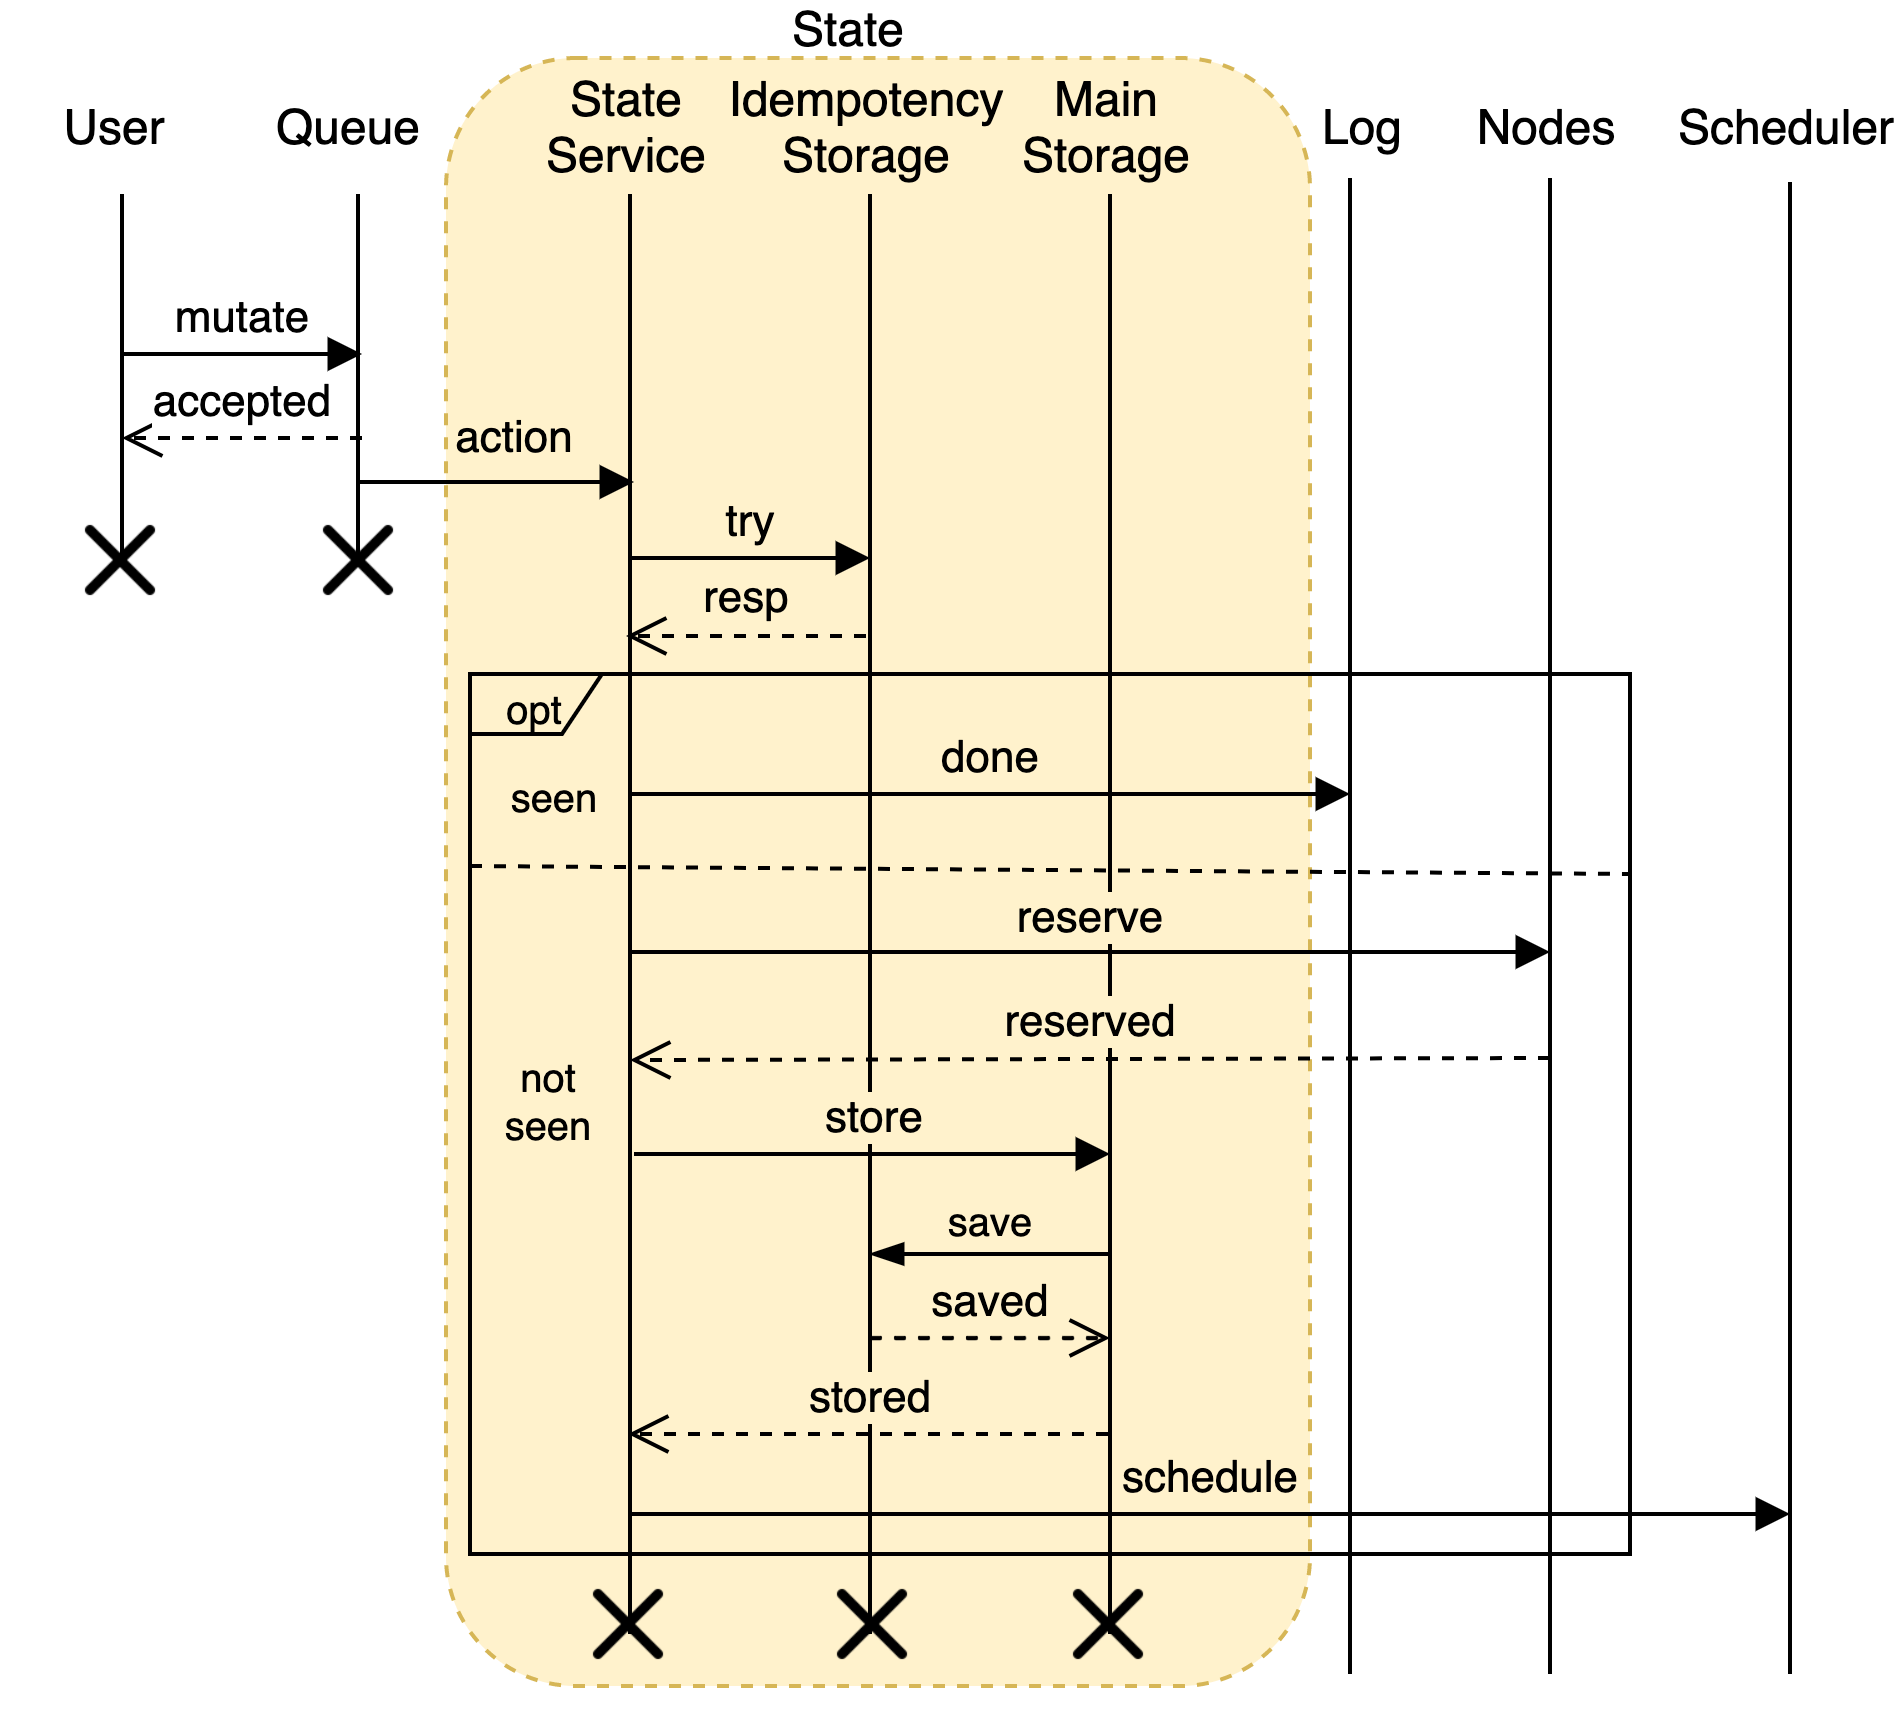
\includegraphics[scale=0.7]{images/Figure13}
	\end{center}
	\vspace{-0.7cm}
	\caption{Low level view of idempotency check communication.}
	\label{fig:fig13}
\end{figure}

The participants follow the communication that we now describe informally: \label{informal_description_idempotency}
\begin{enumerate}[start=1,label={(\bfseries \arabic*)}]
	\item \textbf{User} sends a list request to State service (same as~\ref{sec:cluster_formation_protocol});
	\item \textbf{Queue} accepts the list request and the query local state based on the user selector. If a detail view is required, the state gets metrics data from Nodes service (same as~\ref{sec:cluster_formation_protocol});
	\item \textbf{State service} service that is wrapper aroud system main storage. Interacts with main storage in oreder to create new topologies, regions or clusters, or to get data from main storages about same entities.
	\item \textbf{Idempotency storage} contains idempotent set for all \textbf{already} formed topologies, regions and clusters.
	\item \textbf{Main storage} contains records about desired state for all formed topologies, regions and clusters.
	\item \textbf{Log} contains records of operations. Users can query this service to see if their tasks are finished or have any problems (same as~\ref{sec:cluster_formation_protocol});
	\item \textbf{Nodes} accept messages from State. If possible, it will reserve desired nodes, otherwise it will send an error message to Log service. On a health-check message, if a node is used in some cluster, it will inform that the node is alive (same as~\ref{sec:cluster_formation_protocol});
	\item \textbf{Scheduler} waits for a message sent from State, and pushes clus- ter formation messages to desired nodes (same as~\ref{sec:cluster_formation_protocol});
\end{enumerate}

When testing is request idempotent we must have in mind that stored structure could be $(1)$ \textbf{flat keyspace} and \textbf{$(2)$ hierarhical keyspace} both options are valid as log as \textbf{structure is idempotent} and we can do \textbf{idempotent operation} over that structure. For example $set$ as a data structure and $intersection$ are good candidates. Algorithm that will test structure idempotency must be able to test both options. Algorithm~\ref{alg:alg6} describe steps requred to test if operation is done before.

\begin{algorithm}[H]
	\SetKwFunction{idempotent}{idempotent}
	\SetKwProg{Fn}{function}{:}{}
	\Fn{\idempotent{$stored$, $topology$}}{
		\ForEach{data $\in$ topology}{
			\If{isNotSet(data)}{
				\uIf{stored.intersection(data) = stored}{
					\KwRet{true}
				}
				\KwRet{false}
			}
			\Else{\idempotent{$stored, data$}}
		}
	}
	
	\SetAlgoLined
	\SetKwInOut{Input}{input}
	\Input{request}
	id $\leftarrow$ seenBefore(request.payload.name)\\
	\uIf{id = null}{
		return true;
	}\Else{
		stored $\leftarrow$ storage.findRequest(id)\\
		topology $\leftarrow$ request.payload.topology\\
		\KwRet{\idempotent{$stored, topology$}}
	}
	\caption{Mutate idempotency check}
	\label{alg:alg6}
\end{algorithm}

Next we present a formal description of the idempotency check protocol (cf. Figure~\ref{fig:fig13}) by using~\cite{HuY17}. The global protocol $\G_3$ (given bellow) conforms the informal description given at page~\pageref{informal_description_idempotency}. At this point, the $\mathtt{user}$ can choose one of two possible messages: 

\begin{enumerate}[start=1,label={(\bfseries \arabic*)}]
\item $\mathit{quit}$, in which case the protocol terminates; or, 
\item $\mathit{mutate}$, and the mutation process, described with global protocol $\G'$, starts;
\end{enumerate}

\begin{align*}
\G_3 & = 
\left\{
\begin{array}{@{}l@{}}  
\mathtt{user}\to\mathtt{service}{:} \mathit{quit}().\tend\\
\mathtt{user} \to \mathtt{service}{:}\mathit{create}(\T_3).
\mathtt{state} \to \mathtt{user}{:}\mathit{ok}().\G'
\end{array} \right.
\end{align*}
\myequations{Idempotency check global protocol.}

The mutate protocol $\G'$, activated in the first branch in $\G_3$, starts with $\mathtt{user}$ sending 
$\mathtt{create}$ message to $\mathtt{state}$, specifying also informations about new user desired state typed with $\T_3$, 
and $\mathtt{state}$ replies back with $\mathit{ok}$. This process is the same as cluster formation protocol (cf. section~\ref{cluster_formation_informal_description}). Now we start specific communication protocol for idempotency check so $\mathtt{service}$ sends payload $T_3$ to $\mathtt{istorage}$ to test is this request $seen$ before. The $\mathtt{istorage}$ responds with payload $T_6$ to $\mathtt{service}$, and based on $Boolean$ response $\mathtt{service}$ can do one of two things:

\begin{enumerate}[start=1,label={(\bfseries \arabic*)}]
\item $\mathtt{service}$ sends message to $\mathtt{log}$ and this process terminates; or,
\item $\mathtt{service}$ sends $\mathit{ids}$ of the nodes to be reserved (specified in the payload typed with $\T_4$) to $\mathtt{nodes}$;
\end{enumerate}

\noindent
same as cluster formatoin protocol (cf. section~\ref{cluster_formation_informal_description}). For simplification, we can assume that all nodes are reserved, and now idempotency data store global protocol $\G''$, starts;
\begin{align*}
G' & = 
\mathtt{service} \twoheadrightarrow \mathtt{istorage}{:}\mathit{try}(\T_3). \\
& \hspace{1mm}
\mathtt{istorage} \to \mathtt{service}{:}\mathit{resp}(\mathsf{Boolean}).\\
& \hspace{10mm}
\left\{
\begin{array}{@{}l@{}}
\mathtt{service} \twoheadrightarrow\mathtt{log}{:} \mathit{done}(\mathsf{String}).\tend\\
\mathtt{service} \twoheadrightarrow\mathtt{nodes}{:}\mathit{ids}(\T_4).
\mathtt{nodes} \to \mathtt{service}{:}\mathit{rsrvd}().\G''
\end{array} \right.
\end{align*}

The idempotency store protocol $\G''$, starts with $\mathtt{service}$ sending mutation payload $T_3$ to $\mathtt{mstorage}$. Then $\mathtt{mstorage}$ sends same payload to $\mathtt{istorage}$. When data is saved for future testing, $\mathtt{istorage}$ respond back to $\mathtt{mstorage}$, and finally $\mathtt{mstorage}$ respond back to $\mathtt{service}$. At this poing user payload $T_3$ is stored in both main storage and idempotency storage for future testing. Protocol continue with $\mathtt{state}$ connects $\mathtt{sched}$ (Scheduler) with message $\mathit{ids}$ and the payload that contains other data imported for mutation to be completed (typed with $\T_5$), and the rest of cluster formation protocol may continue.

\begin{align*}
\G'' = & 
\mathtt{service} \twoheadrightarrow \mathtt{mstorage}{:}\mathit{store}(\T_3).
\mathtt{mstorage} \twoheadrightarrow \mathtt{istorage}{:}\mathit{save}(\T_3).\\
& \hspace{4mm}
\mathtt{istorage} \to \mathtt{mstorage}{:}\mathit{saved}().
\mathtt{mstorage} \to \mathtt{service}{:}\mathit{stored}().\\
& \hspace{4mm}
\mathtt{service} \twoheadrightarrow \mathtt{sched}{:}\mathit{ids}(\T_5).\tend
\end{align*}

We may now obtain the projections of global type $\G_3$ onto the participants $\mathtt{user}, \mathtt{service}, \mathtt{istorage}$, $\mathtt{mstorage}$, $\mathtt{log}$, $\mathtt{nodes}$: and $\mathtt{sched}$:

\begin{align*}
\ST_\mathsf{user} = &
{+}
\left\{
\begin{array}{@{}l@{}}
\mathtt{service}{!}\mathit{quit}().\tend\\
\mathtt{service}{!}\mathit{create}(\T_3).\mathtt{service}{?}\mathit{ok}().\tend\\
\end{array} \right.
\end{align*}
\begin{align*}
	\ST_\mathsf{service} = &
	{+}
	\left\{
	\begin{array}{@{}l@{}}
	\mathtt{user}{?}\mathit{quit}().\tend \\
	\mathtt{user}{?}\mathit{create}(\T_3).\mathtt{user}{!}\mathit{ok}().\ST'\\
	\end{array} \right.
\end{align*}
where
\begin{align*}
	\ST' = &
	\mathtt{istorage}{!!}\mathit{try}(\T_3).\mathtt{istorage}{?}\mathit{resp}(\mathsf{Boolean}).\\
	&
	{+}
	\left\{
	\begin{array}{@{}l@{}}
	\mathtt{log}{!!}\mathit{done}(\mathsf{String}).\tend\\
	\mathtt{nodes}{!!}\mathit{ids}(\T_4).\mathtt{nodes}{?}\mathit{rsrvd}().\ST''\\
	\end{array} \right.
\end{align*}
\begin{align*}
	\ST_\mathtt{mstorage} =  & \hspace{2mm}
	\mathtt{service}{??}\mathit{store}(\T_3).\mathtt{istorage}{!!}\mathit{save}(\T_3).\\ & \hspace{-8mm}
	\mathtt{istorage}{?}\mathit{saved}().\mathtt{service}{!}\mathit{stored}().\tend
\end{align*}
\begin{align*}
	\ST'' = & 
	\mathtt{mstorage}{!!}\mathit{store}(\T_3).\mathtt{mstorage}{?}\mathit{stored}().\\ & \hspace{-8mm}
	\mathtt{sched}{!!}\mathit{ids}(\T_5).\tend
	%\end{align*}
	%
	%\begin{align*}
\end{align*}
\begin{align*}
	\ST_\mathtt{istorage} =  &
	\mathtt{service}{??}\mathit{try}(\T_3).\mathtt{service}{!}\mathit{resp}(\mathsf{Boolean}).\\ & \hspace{-8mm}
	\mathtt{mstorage}{??}\mathit{save}(\T_3).\mathtt{mstorage}{!}\mathit{saved}().\tend
\end{align*}
\begin{align*}
	\ST_\mathtt{log} =  &
	\mathtt{service}{??}\mathit{done}(\mathsf{String}).\tend
\end{align*}
\begin{align*}
	\ST_\mathtt{nodes} =  &
	\mathtt{service}{??}\mathit{ids}(\T_4).\mathtt{service}{!}\mathit{rsrvd}().\tend
\end{align*}
\myequations{Idempotency check global protocol projection.}
Similarly as for $\G_2$ we remark $\G_3$ could also be modeled using standard MPST (e.g.,~\cite{HondaYC08}), but again the projection types would be undefined, while following the approach of ~\cite{HuY17} with explicit connections, we have obtained all valid projections.
%
%
\subsection{List detail protocol}\label{sec:list_detail_protocol}
%
The last communication protocol in our system appears in the information retrieval process. Namely, on formed topologies, using labels, the user can specify what part of the system he wants to retrieve, for example to visualise on some dashboard. Two options are available: 

\begin{enumerate}[start=1,label={(\bfseries \arabic*)}]
	\item \textbf{global view} of the system --- all topologies the user manages
	\item \textbf{specific clusters} details --- complete details about specified clusters like resources utilization over time (using stored metrics information), node information, and running or stopped services.
\end{enumerate}

It is important to note, that similar to the query operation, both rules $(\ref{eq:eq1})$ and $(\ref{eq:eq2})$ must be satisfied in order for information to be present in the response. 

One additional information may be specified is whether the user wants a detailed view or not. If detail view information is presented in a request, the user will get a detailed view. 

Figure \ref{fig:fig8}. shows a low-level view of the list operation protocol, where users can get details about the formed system. In this setting, the system involves participants: User, State, Nodes, and Log. 

\begin{figure}[!htbp]
	\begin{center}
		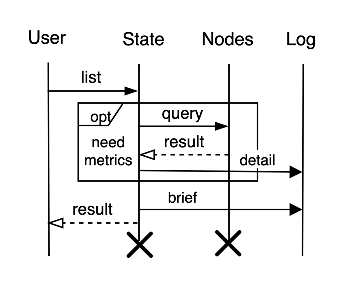
\includegraphics[scale=0.9]{images/FIG4}
	\end{center}
	\vspace{-1.2cm}
	\caption{Low level view of list operation communication.}
	\label{fig:fig8}
\end{figure}

We now informally describe the participants roles in the protocol:\label{list_protocol_informal_description}

\begin{enumerate}[start=1,label={(\bfseries \arabic*)}]
	\item \textbf{User} sends a list request to State service;
	\item \textbf{State} accepts the list request and the query local state based on the user selector. If a detail view is required, the state gets metrics data from Nodes service;
	\item \textbf{Nodes} contain node metrics data, and if required, it may send this data to State;
	\item \textbf{Log} contains records of all operations. Users can query this service.
\end{enumerate}

Algorithm \ref{alg:alg5} describes steps after the state receives a list message.

\begin{algorithm}[H]
	\SetAlgoLined
	\SetKwInOut{Input}{input}
	\Input{request}
	Initialize: data $\leftarrow$ []\\
	\ForEach{(topology, isDetail) $\in$ userData(request.query)}{
		\uIf{isDetail}{
			data.append(topology.collectData())\\
		}\Else{
			data.append(topology.data())\\
		}
	}
	\Return data
	\caption{List of current state of the system}
	\label{alg:alg5}
\end{algorithm}

Next we present a formal description of the list communication protocol (cf. Figure \ref{fig:fig4}) by using~\cite{HuY17}.
Global type $\G_4$ (given below) starts with $\mathtt{user}$ connecting $\mathtt{state}$ with one of the two possible messages: 
$(1)$ $\mathit{list}$, specifying a request for a detailed view, where sort $\T_1$ identifies which parts of the system user wants to view in details, after which $\mathtt{state}$ connects $\mathtt{nodes}$ with $\mathit{query}$ message, with a payload of sort $\T_2$  containing specification of which nodes need to show their metrics data, and then protocol proceeds as prescribed with $\G'$; 
$(2)$ $\mathit{list^*}$, specifies no need for a detailed view is specified, where a payload of sort $\T_4$ denotes user specified parts of the system the user wants to view, but without greater details. In the latter case protocol follows global type $\G''$.
\begin{align*}
\G_4 &= 
\left\{
\begin{array}{@{}l@{}}  
\mathtt{user} \twoheadrightarrow \mathtt{state}{:}\mathit{list}(\T_1).\mathtt{state}\twoheadrightarrow\mathtt{nodes}{:}\mathit{query}(\T_2). \G' \\
\mathtt{user} \twoheadrightarrow \mathtt{state}{:}\mathit{list^*}(\T_4).\G''
\end{array} \right.
\end{align*}
\myequations{List detail global protocol.}
Global type $\G'$ starts with $\mathtt{nodes}$ replying to $\mathtt{state}$ $\mathit{result}$ message and a payload identifying parts of the system user wants to see in greater detail typed with $\T_3$. Then, $\mathtt{state}$ connects $\mathtt{log}$ with $\mathtt{details}$ and also sends $\mathtt{result}$ to $\mathtt{user}$, and finally terminates. 
In $\G''$, $\mathtt{state}$ also connects $\mathtt{log}$ with $\mathit{brief}$ and a payload typed with $\T_5$ identifying parts of the system user wants to see without greater detail. Then, $\mathtt{state}$ replies to $\mathtt{user}$ with $\mathtt{result}$ message, and the protocol terminates.
\begin{align*}
\begin{split}
	\G' =  & 
	\mathtt{nodes}\to\mathtt{state}{:}\mathit{result}(\T_3).\mathtt{state}\twoheadrightarrow \mathtt{log}{:}\mathit{detail}(\T_3). \\
	& \hspace{2mm}
	\mathtt{state}\to\mathtt{user}{:}\mathit{result}(\T_3).\tend
\end{split}
\end{align*}
\begin{align*}
	\G'' = &
	\mathtt{state}\twoheadrightarrow \mathtt{log}{:}\mathit{brief}(\T_5).\mathtt{state}\to\mathtt{user}{:}\mathit{result}(\T_5).\tend
\end{align*}

Same as for the health-check and the cluster formation protocols, here we also present the projections of global type $\G_4$, modeling the list protocol, onto participants $\mathtt{user}$, $\mathtt{state}$, $\mathtt{nodes}$, and $\mathtt{log}$:
\begin{align*}
	\ST_\mathtt{user} =& 
	{+}
	\left\{
	\begin{array}{@{}l@{}}  
	\mathtt{state}{!!}\mathit{list}(\T_1).\mathtt{state}{?}\mathit{result}(\T_3).\tend \\
	\mathtt{state}{!!}\mathit{list^*}(\T_4).\mathtt{state}{?}\mathit{result}(\T_5).\tend 
	\end{array} \right.
\end{align*}
\begin{align*}
	\ST_\mathtt{state} =&
	{+}
	\left\{
	\begin{array}{@{}l@{}}  
	\mathtt{user}{??}\mathit{list}(\T_1).\mathtt{nodes}{!!}\mathit{query}(\T_2).\ST'\\
	\mathtt{user}{??}\mathit{list^*}(\T_4).\mathtt{log}{!!}\mathit{brief}(\T_5).\mathtt{user}{!}\mathit{result}(\T_5).\tend
	\end{array} \right. 
\end{align*}
where
\begin{align*}
	\ST'  =& 
	\mathtt{nodes}{?}\mathit{result}(\T_3).\mathtt{log}{!!}\mathit{detail}(\T_3).\mathtt{user}{!}\mathit{result}(\T_3).\tend
\end{align*}
\begin{align*}
	\ST_\mathtt{nodes} = &
	\mathtt{state}{??}\mathit{query}(\T_2).\mathtt{state}{!}\mathit{result}(\T_3).\tend
\end{align*}
\begin{align*}
	\ST_\mathtt{log} = & 
	{+}
	\left\{
	\begin{array}{@{}l@{}}  
	\mathtt{state}{??}\mathit{detail}(\T_3).\tend \\
	\mathtt{state}{??}\mathit{brief}(\T_5).\tend \\
	\end{array} \right.
\end{align*}
\myequations{List detail global protocol projection.}
For instance, type $\ST_\mathtt{log}$ specifies $\mathtt{log}$ gets included in the session only after receiving from $\mathtt{state}$, either message $\mathit{detail}$, or message $\mathit{brief}$, and then terminates. 

Similarly as for $\G_2$ and $\G_3$ we remark $\G_4$ could also be modeled using standard MPST (e.g.,~\cite{HondaYC08}), but again the projection types would be undefined, while following the approach of ~\cite{HuY17} with explicit connections, we have obtained all valid projections.
%
%
\section{Access pattern}\label{sec:access_pattern}
%
In section~\ref{sec:application_model}, we already disccus system accesspattern from applications point of view, using streams and topics. In this section we are going to venture in dashboard and system access described in~\ref{sec:distribution_models}. 

To acces the system, requests are going over some \textit{master process}. This process is not responsable to any sort of synchronization, agreement or something like that, but just to show dashboards and various system details since cloud is avalible anywhere in the world, while micro-cloud should serve local population. 

One question that could come to the mind is, what if some cloud provider offering micro-cloud functionality, or running our master process goes down, should rest of the micro-clouds go to \textit{read-only} mode and only accept \textbf{read} requests?

All communication is not exclusive to go over that master process, but if user is nearby to micro-cloud should be able initiate commands direcly to clusters, regions and topologies. But for dashboards and full informations about his micro-clouds cloud would be better solution, just because of more avalibe resources.

If some cloud provider goes down for whatever reason, we should foreseen this and to resolve it we could use multiple cloud providers using \textit{Multi-Cloud Computing}~\cite{HongDSH19, Ardagna15}, so that one cloud provider is master process and many others are backup in case the whole cloud provider goes down.

Here inevitably we have some state synchornization, and here we could rely on SEC and CRDTs to do synchrnoization without some expensive coordination between providers.

This is not generally a problem, if applicatoins that are running in micro-clouds are not dependent on some process, location, sensors od services etc. If we this is the case, than we can connect micro-clouds in sort of P2P network and give them some logic to just route request to proper location on the globe. 

This might not be that fast, since even light is afected by the distance, but we would be able to issue requests to cluster on totally different part of the world.
%
%
\section{Repercussion}\label{sec:repercussion}
%
Model presented in this chapter, have two possible repercussions:

\begin{enumerate}[start=1,label={(\bfseries \arabic*)}]
	\item \textbf{Stand alone}, the proposed model can serve as a base layer for future ECC as a service implementation. On top of it, we can implement other services and features like scheduling, storage, applications, management, monitoring, etc. As such it could be valiable option in the CC.
	\item \textbf{Integration}, the proposed model could be integrated with existing systems like Kubernetes, OpenShift, or cloud provider infrastructure since they all operate over the cluster. This is possible, with some small infrastructure changes and adaptations because --- the communication should implemented via standard interfaces like HTTP and JSON, the integrations should be relatively easy to achieve. The proposed model could be used as a geo-distributed description and/or an  organization tool.
\end{enumerate} 
%
%
\section{Limitations}\label{sec:limitations}
%
Since the perfect model never existed, model that is proposed in this thesis have some limitations, that we must be aware of. Either to work on improvements, or use the model as is. 

When talking about small scale servers and micro-clouds, we must be aware of the few things. 

\begin{enumerate}[start=1,label={(\bfseries \arabic*)}]
	\item not all companies and organizations will be able to deploy them, due to the high investments required~\cite{MonsalveCC18}. Similar to the cloud where massive DCs are built by a few companies and used by many others. These small servers could be deployed by government authorities or large cloud companies for their own needs. The general public can use them, similarly to the cloud --- pay as you go, model.
	\item there is no guarantiee that existing public cloud providers will allow nodes that are not built, resigned or deployed by them. If we are building private cloud, thant we can make different decision. One way to resolve this issue is that whole platform become open-source, so that public cloud providers can engage into development, and eventually use tham as a solution.
	\item These small scale servers must be out of reach of people, and protected in some way so that not everyone have access to them. Some degree of phisical security mut be implemented.
	\item places where these small scale servers will be deployd must have stable internet connection, and ability to integrate SDN or other similar techologies, so that complex network topologies could be implemented properly.
	\item these servers can have some open architecture or could be custom built by other providers. In both cases they must be able to satisfy rules that are presented in~\ref{sec:separation_of_concerns}.
	\item spliting into two parts processing and possibility that users can be responsabile for micro-clouds may rise some legal concerns. Either to develop interesting applications, use tham as a firewall or simply use them as a privacy level for data there must be legal agreement that might not be that easy to achieve.
\end{enumerate}
%
%